% =========================================================
% MÓDULO DE PERSISTENCIA (BASE DE DATOS)
% =========================================================
\chapter{Modelo de Persistencia}
\label{cap:diseno_persistencia}
En este capítulo se detalla la arquitectura de datos del sistema, incluyendo el diseño lógico y físico de la base de datos, así como las estrategias implementadas para garantizar la integridad y seguridad de la información.

\section{Diagrama Entidad-Relación (DER)}
El diseño del modelo de datos sigue un enfoque relacional. A continuación se presenta la representación gráfica del modelo físico, el cual detalla las entidades, sus atributos y las relaciones de cardinalidad que rigen el flujo de información.
\begin{figure}[htbp]
    \centering
    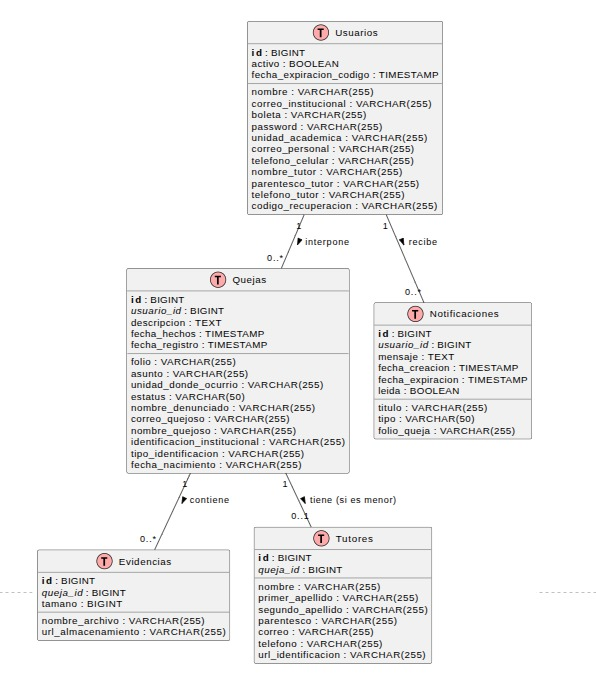
\includegraphics[width=0.9\textwidth]{imagenes/quejoso/basededatosquejoso.png} 
    \caption{Diagrama de Entidad-Relación del Sistema de Denuncia.}
    \label{fig:der_sistema}
\end{figure}

\section{Diccionario de Datos}
El diccionario de datos proporciona una descripción técnica exhaustiva de cada tabla en el sistema.

\subsection{Tabla: Usuarios}
Almacena los datos de identidad y acceso de los quejosos y administradores.

\begin{table}[htbp]
\centering
\small
\begin{tabular}{|l|l|l|p{6cm}|}
\hline
\rowcolor[HTML]{EFEFEF} 
\textbf{Campo} & \textbf{Tipo} & \textbf{Restricción} & \textbf{Descripción} \\ \hline
id & BIGINT & PK, NOT NULL & Identificador único interno. \\ \hline
correo\_institucional & VARCHAR(255) & UNIQUE, NOT NULL & Correo oficial para autenticación y contacto. \\ \hline
boleta & VARCHAR(255) & UNIQUE & Identificador académico del alumno. \\ \hline
password & VARCHAR(255) & NOT NULL & Contraseña cifrada (BCrypt). \\ \hline
activo & BOOLEAN & DEFAULT TRUE & Estado de habilitación de la cuenta. \\ \hline
\end{tabular}
\caption{Diccionario de datos de la tabla Usuarios.}
\end{table}

\subsection{Tabla: Quejas}
Entidad núcleo del sistema que registra los detalles de cada denuncia.

\begin{table}[htbp]
\centering
\small
\begin{tabular}{|l|l|l|p{6cm}|}
\hline
\rowcolor[HTML]{EFEFEF} 
\textbf{Campo} & \textbf{Tipo} & \textbf{Restricción} & \textbf{Descripción} \\ \hline
id & BIGINT & PK, NOT NULL & Identificador único de la queja. \\ \hline
usuario\_id & BIGINT & FK, NOT NULL & Referencia al usuario denunciante. \\ \hline
folio & VARCHAR(255) & UNIQUE, NOT NULL & Código alfanumérico para seguimiento público. \\ \hline
estatus & VARCHAR(50) & NOT NULL & Estado actual (e.g., PENDIENTE, EN\_REVISION). \\ \hline
fecha\_registro & TIMESTAMP & NOT NULL & Fecha de creación automática del registro. \\ \hline
\end{tabular}
\caption{Diccionario de datos de la tabla Quejas.}
\end{table}

\section{Estrategia de Persistencia}
La persistencia de datos se gestiona mediante las siguientes definiciones tecnológicas:
\begin{itemize}
    \item \textbf{Motor de Base de Datos:} Se utiliza un motor relacional (\textbf{PostgreSQL/MySQL}) para asegurar el cumplimiento de las propiedades ACID y la integridad referencial mediante claves foráneas.
    \item \textbf{Mapeo Objeto-Relacional (ORM):} Se emplea \textbf{Hibernate} a través de \textbf{Spring Data JPA}. Esto permite manipular los datos como objetos Java, reduciendo la probabilidad de errores en consultas SQL manuales.
    \item \textbf{Patrón Repository:} Se implementó este patrón para abstraer la capa de datos, facilitando la mantenibilidad y el intercambio de motores de base de datos en el futuro.
\end{itemize}

\section{Scripts de Creación (DDL)}
A continuación se presenta el script fundamental para la generación de la tabla de quejas:

\begin{verbatim}
CREATE TABLE quejas (
    id BIGINT PRIMARY KEY GENERATED ALWAYS AS IDENTITY,
    usuario_id BIGINT REFERENCES usuarios(id),
    folio VARCHAR(255) UNIQUE NOT NULL,
    asunto VARCHAR(255) NOT NULL,
    estatus VARCHAR(50) DEFAULT 'PENDIENTE',
    fecha_registro TIMESTAMP DEFAULT CURRENT_TIMESTAMP
);
\end{verbatim}

\section{Seguridad y Rendimiento}
\begin{itemize}
    \item \textbf{Cifrado:} Los datos sensibles como la contraseña se protegen mediante el algoritmo de hash robusto \textbf{BCrypt}.
    \item \textbf{Índices:} Se han creado índices sobre las columnas \texttt{folio} y \texttt{boleta} para optimizar la velocidad de búsqueda en procesos con grandes volúmenes de datos.
\end{itemize}